\documentclass[12pt,a4paper]{report}

\usepackage[english]{babel}
\usepackage[cp1250]{inputenc} 
   % by u�y� polskich znak�w w systemach Linux
   % u�ywamy kodowania "latin2" lub "utf8", dla Windows "cp1250" 
\usepackage{graphicx}
\usepackage{gauss}
\usepackage{amsmath}
\usepackage{tikz}
\usepackage{float}


\newcommand*\circled[1]{\tikz[baseline=(char.base)]{
            \node[shape=circle,draw,inner sep=2pt] (char) {#1};}}
%-------------------------------------------------------------------------------
% TITLE PAGE
%-------------------------------------------------------------------------------

\begin{document}


\title{ \normalsize \textsc{Real Time Operating Systems}
        \\ [1.0cm]
        \line(1,0){350}
        \newline
      \LARGE \textbf  {Final Report}     \line(1,0){350}}
     \date{28.05.2018}
   
   \author{
        Wojciech Juszczak \\
        Jaros�aw Szumega\\
        Adam Superczy�ski }
        
\maketitle
\tableofcontents
\newpage

\newpage
\chapter{Introduction}
The aim of the project was building automatic, self-driving robot with ability to detect and avoid obstacles. System was implemented on STM32 with the use of FreeRTOS.
\newline
General architecture diagram of project is presented below.
\newline
\begin{figure}[h!]
  \caption{Architecture diagram}
  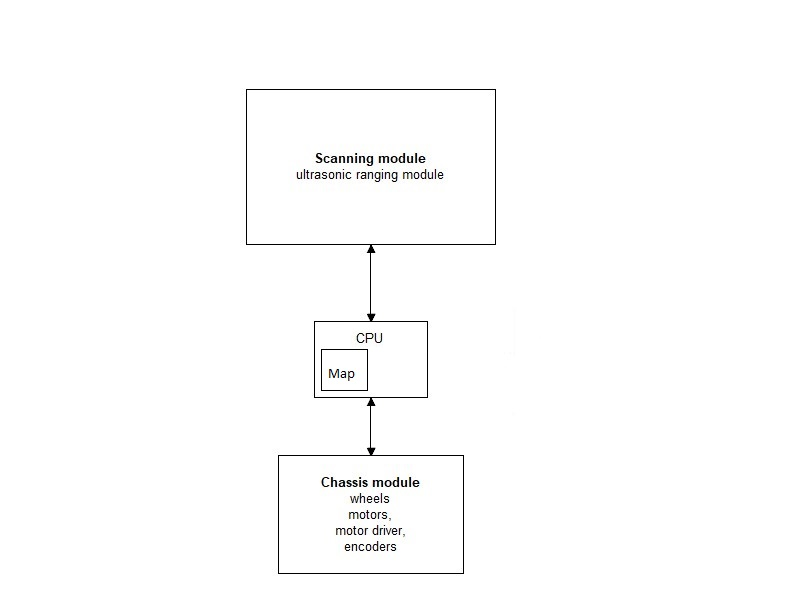
\includegraphics[width=1\textwidth]{architecture_diagram}
\end{figure}
\newline
The whole architecture can be divided into three elements:
\begin{itemize}
  \item Scanning module - used for surrounding scanning and informing about distance to obstacle,
  \item Map - information about surrounding stored inside CPU memory. Based on it robot makes decision about next movement,
  \item Chasis module - deciding about movement, controlling motors  \ldots
\end{itemize}
\chapter{Detailed description of project}
\section{Scanning module}
For this purpose proximity sensor HCSR-04 is used. To start measuring it needs 10us pulse on pin TRIG. After that it will response with pulse on ECHO pin which has width proportional to the distance. High priotity task activates measurement by clearing the timer and setting high signal on TRIG pin. Task becomes blocked and waits for interrupt from ISR. After 10us there is timer interrupt in which signal on TRIG pin is set to low. Next, values of timer in rising and falling edges are saved. On falling edge notification is sent to task. After receiving notification distance is calculated and saved to mutex - locked global variable. Task is blocked for 100ms before next measurement.
\end{document}